\documentclass[11pt]{article}

\usepackage{graphicx}
\usepackage{epstopdf}
\hoffset        2mm 
\voffset        -15mm
\oddsidemargin  0mm
\topmargin      0.5in
\textwidth      6in
\textheight     9in

\begin{document}

\begin{titlepage}

\vspace*{55mm}
\begin{center}
{\huge MATH609-600}\\[1cm]
{\em \huge Programming Assignment \#1}\\[70mm]
{\large Fall, 2015} \\[15mm]
\end{center}

\begin{flushright}
{\LARGE Hasan Tahir Abbas}
\end{flushright}

\vfill

\end{titlepage}

\newpage
\section{Problem Specifications}
The computational exercises explore the appicability of the methods to compute the numerical solutions of linear systems.


\subsection{Exercise 1: System with a Tridiagonal matrix}

The approximate solution of the given linear system is computed and then compared with the exact solution.

\subsection{Exercise 2: Approximation of 2D Elliptic equation}

A 5-point finite difference formula is used to model the two-dimensional elliptic equation. The approximate solution is computed by applying the given boundary conditions.

\subsection{Exercise 3: Hilbert matrix test}

 The versatility of the method developed is tested on an ill-conditioned matrix. 

\bigskip

\section{Preliminaries}

The exercises in this programming assignment utilize the row-based Doolittle Algorithm for LU Factorization where the diagonal elements of the lower triangular matrix L are set to 1. The solution vectors are then found by completing the LU Factorization process. 



\newpage

\section{Computational Results}

\subsection{Exercise 1: System with a Tridiagonal matrix}
%Problem 1 (Hilbert Matrix System)}

\begin{figure}[!hbt]
\begin{center}
	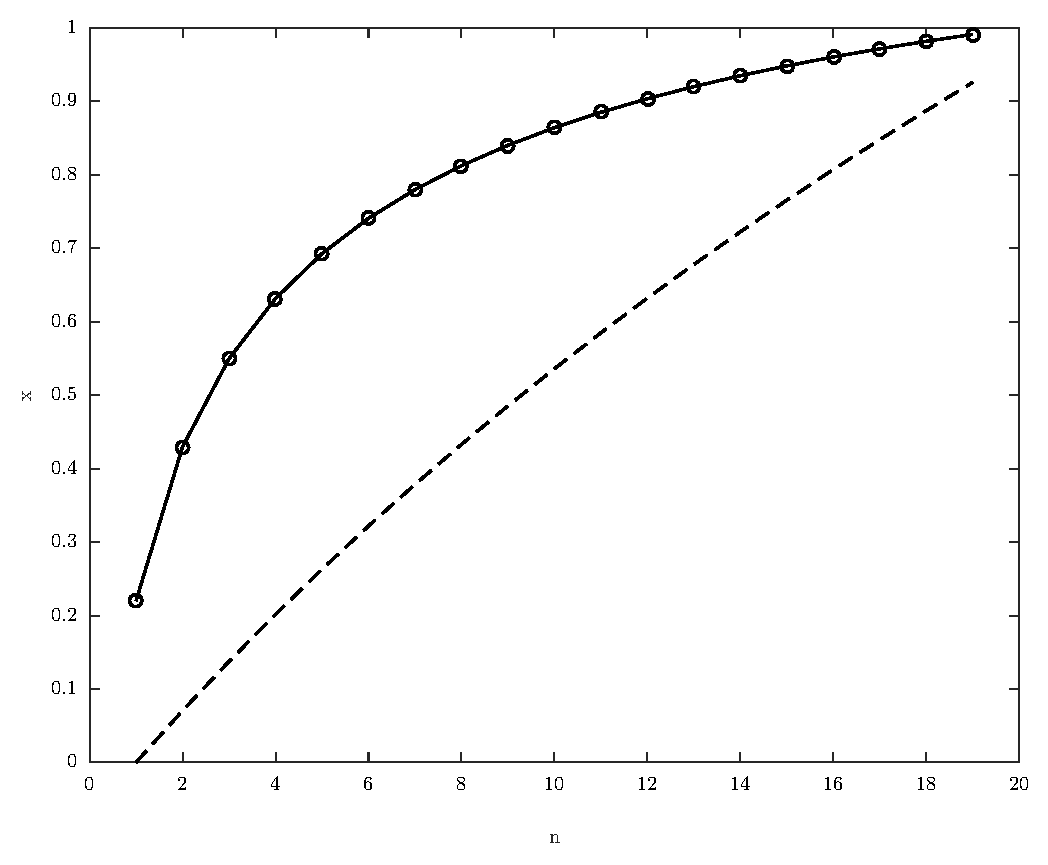
\includegraphics[width=4in]{math609_pa1_comp_example_1_n_19.eps}
	\caption{Approximate solution of FVM based linear system at n = 19}
\end{center}
\end{figure}

\begin{figure}[!hbt]
\begin{center}
	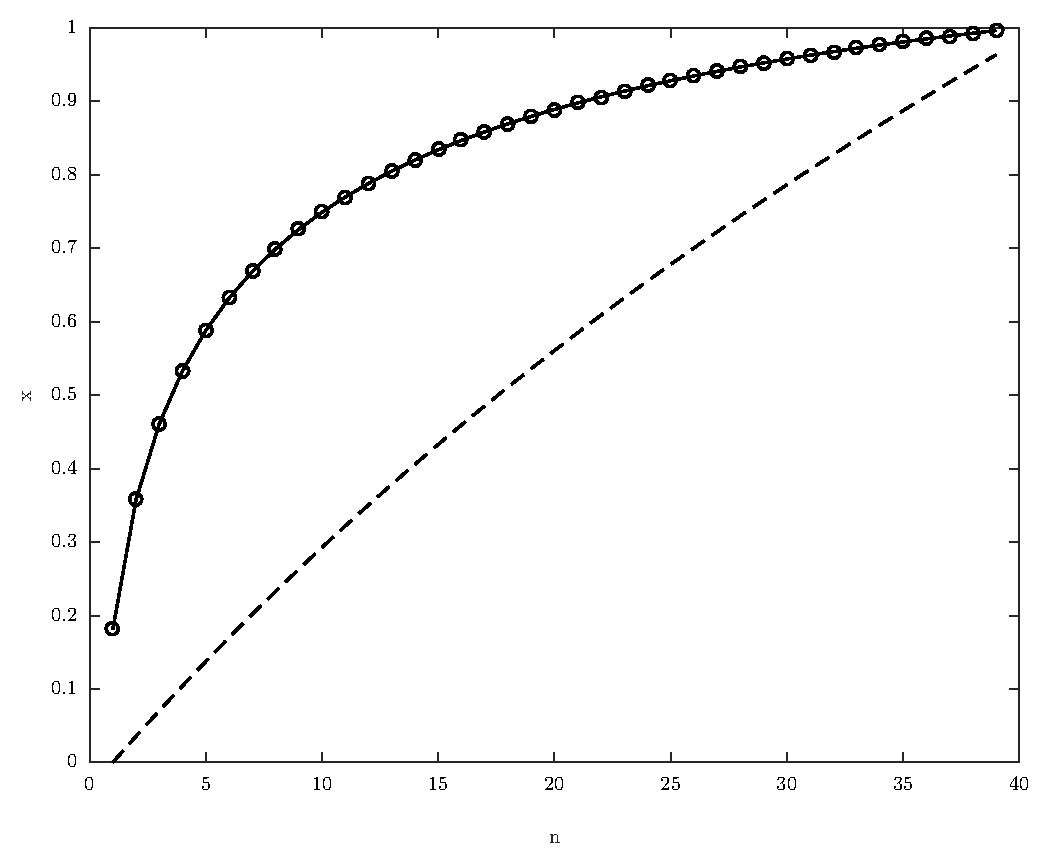
\includegraphics[width=4in]{math609_pa1_comp_example_1_n_39.eps}
	\caption{Approximate solution of FVM based linear system at n = 39}
\end{center}
\end{figure}

\begin{figure}[!hbt]
\begin{center}
	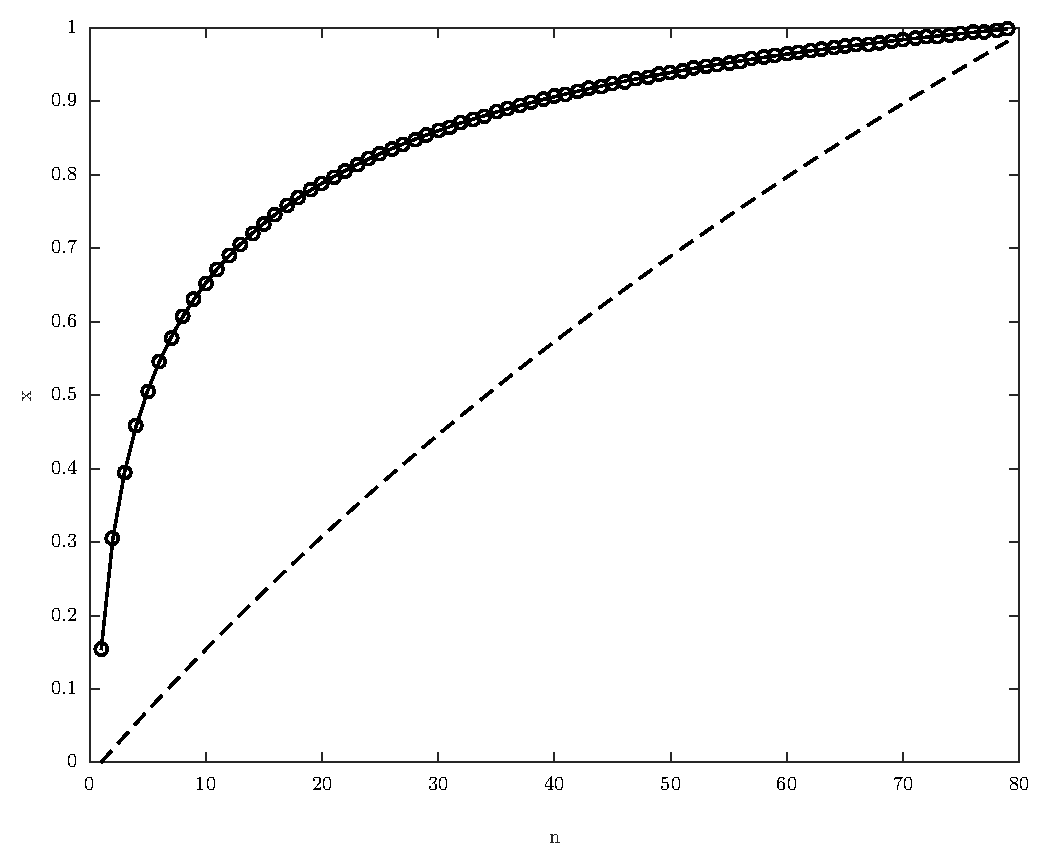
\includegraphics[width=4in]{math609_pa1_comp_example_1_n_79.eps}
	\caption{Approximate solution of FVM based linear system at n = 79}
\end{center}
\end{figure}

\begin{figure}[!hbt]
\begin{center}
	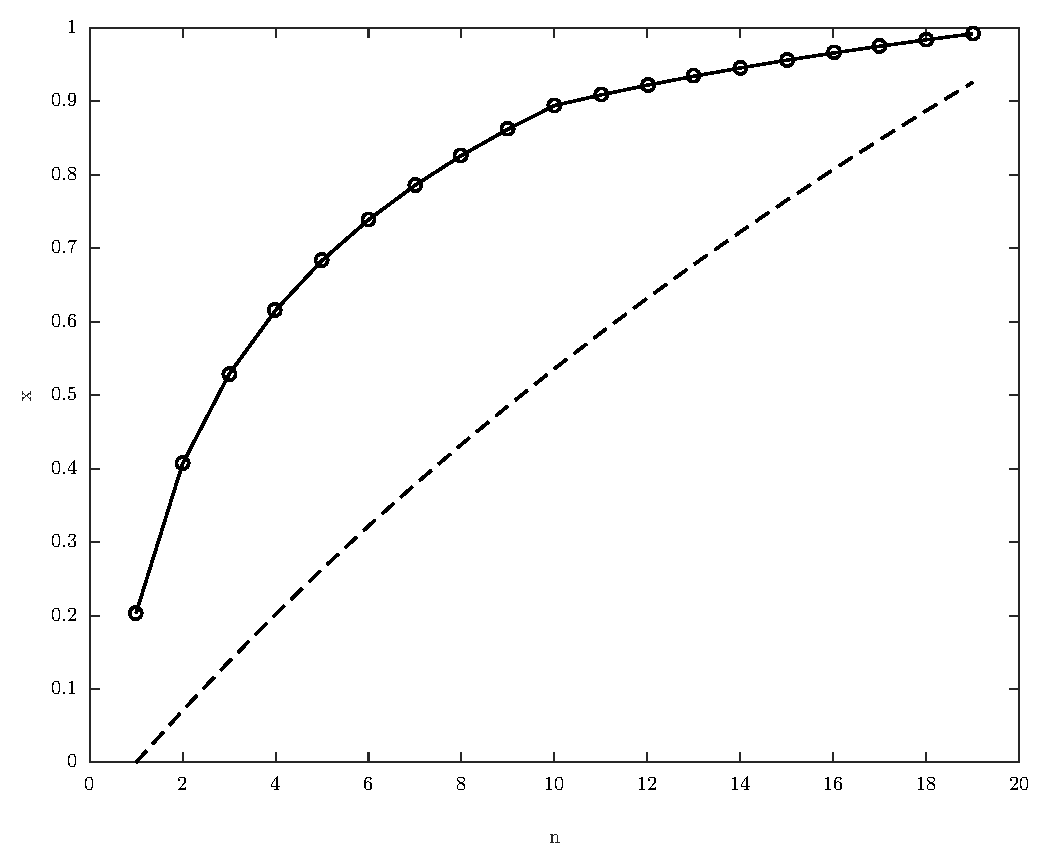
\includegraphics[width=4in]{math609_pa1_comp_example_1_n_19_k_2.eps}
	\caption{Approximate solution of FVM based linear system at n = 19 and K = 2}
\end{center}
\end{figure}

\begin{figure}[!hbt]
\begin{center}
	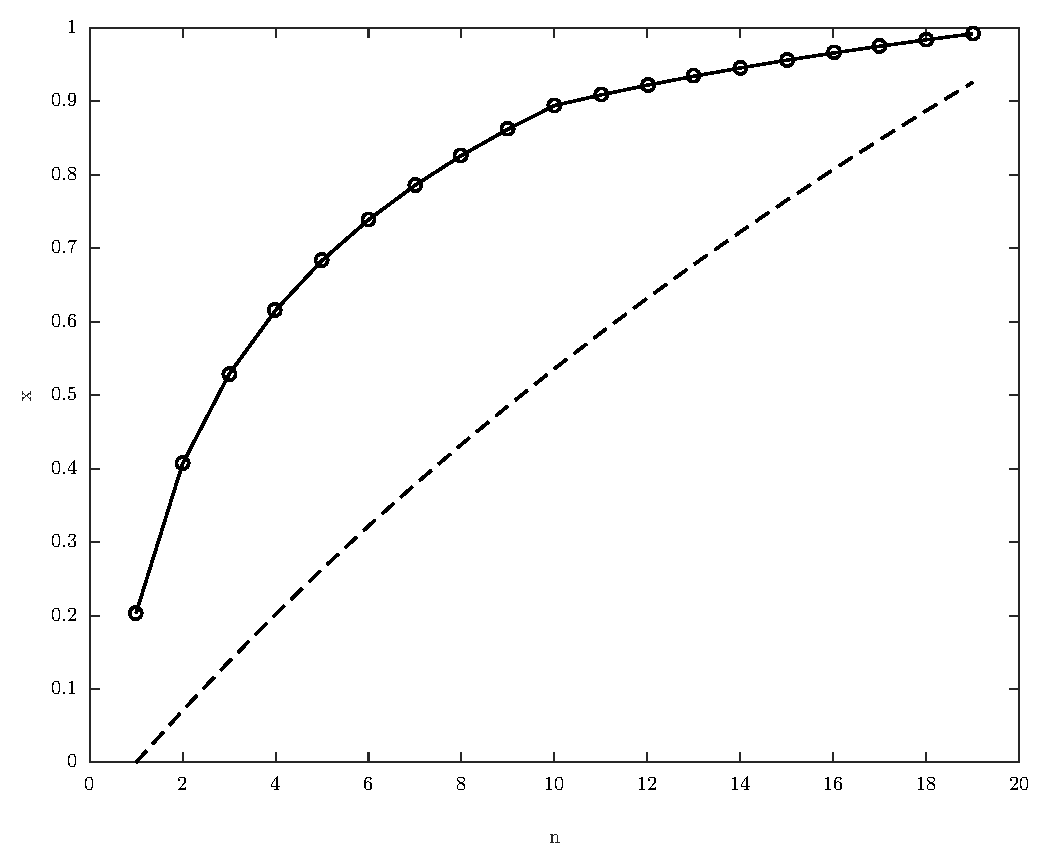
\includegraphics[width=4in]{math609_pa1_comp_example_1_n_19_k_2.eps}
	\caption{Approximate solution of FVM based linear system at n = 19 and K = 5}
\end{center}
\end{figure}

\begin{figure}[!hbt]
\begin{center}
	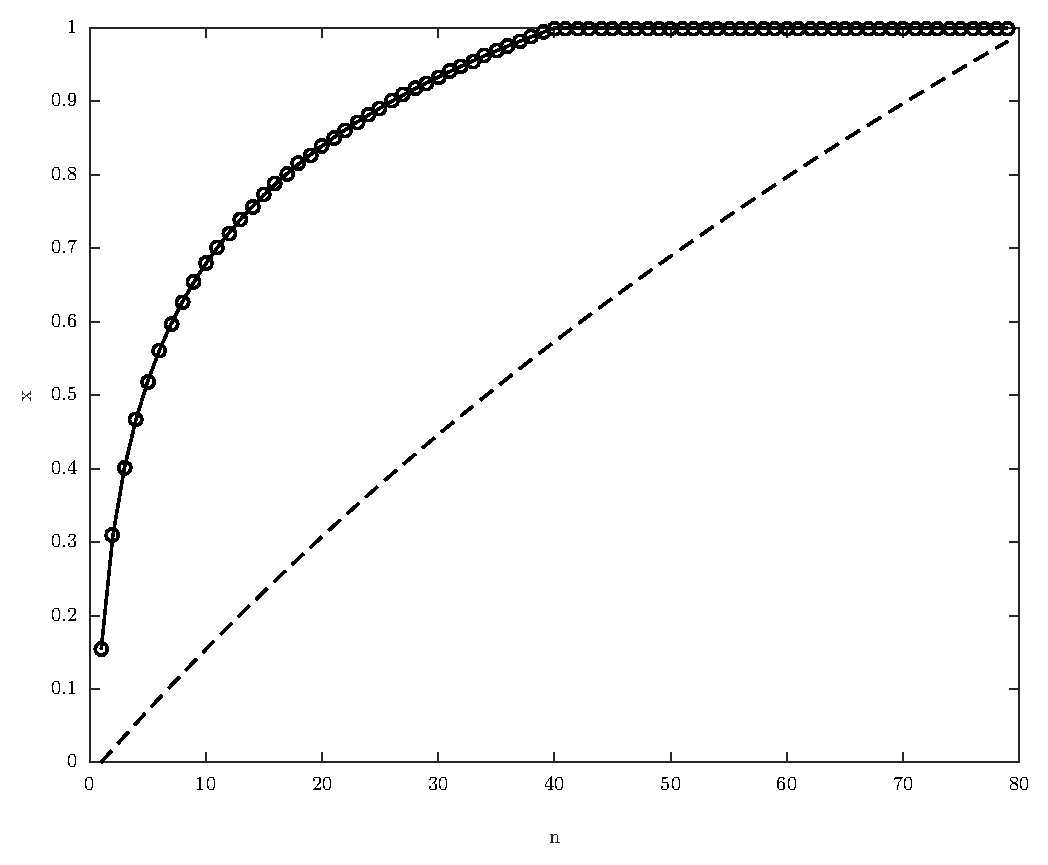
\includegraphics[width=4in]{math609_pa1_comp_example_1_n_79_k_1000.eps}
	\caption{Approximate solution of FVM based linear system at n = 79 and K = 1000}
\end{center}
\end{figure}

\subsection{Exercise 2: Approximation of 2D Elliptic equation}

\begin{figure}[!hbt]
\begin{center}
	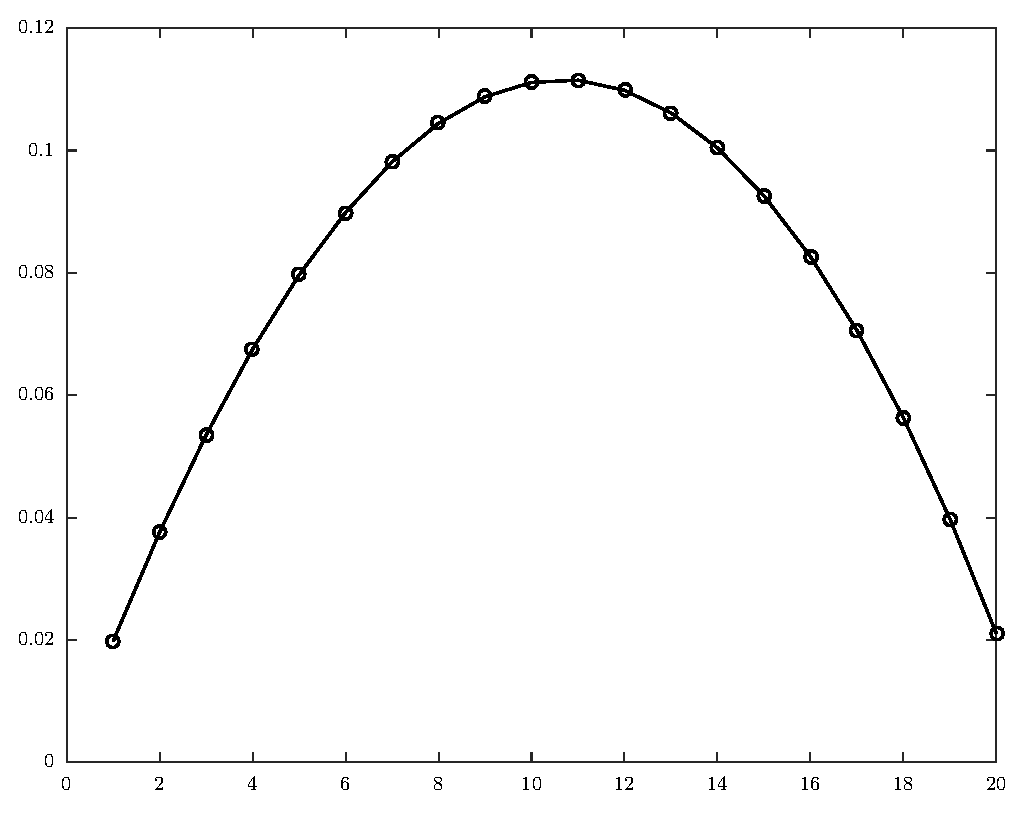
\includegraphics[width=4in]{math609_pa1_comp_example_2_n_20.eps}
	\caption{Approximate solution of 5-point elliptic equation at n = 20}
\end{center}
\end{figure}

\begin{figure}[!hbt]
\begin{center}
	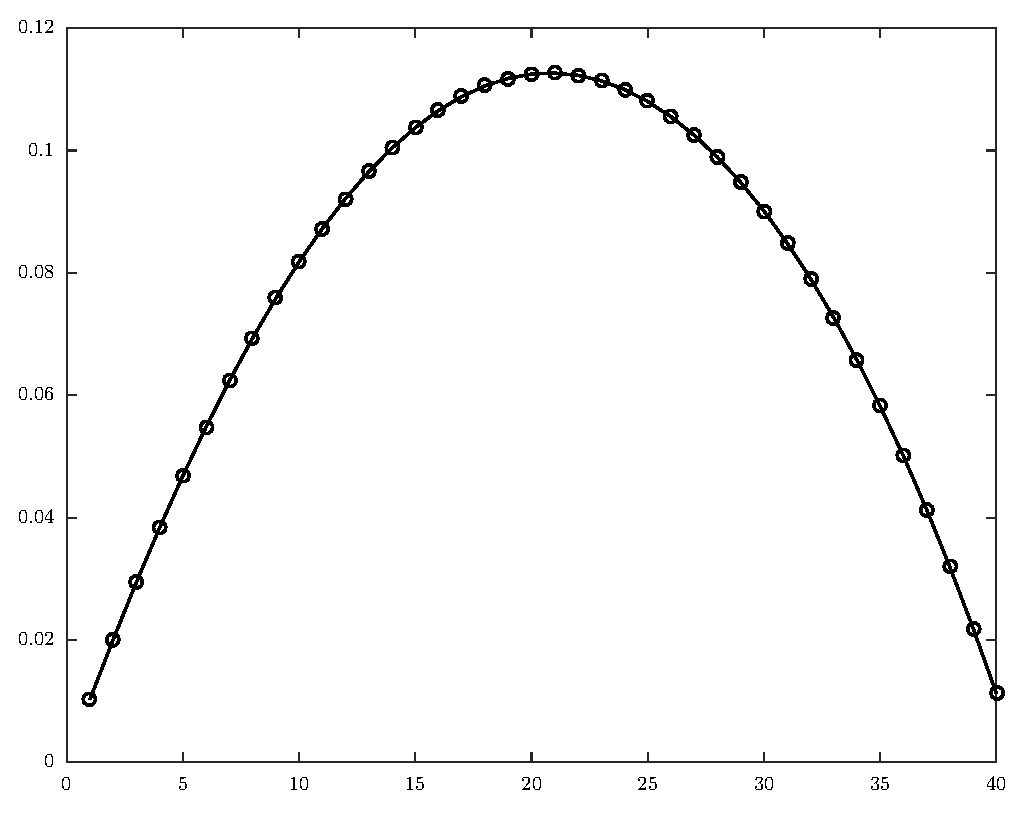
\includegraphics[width=4in]{math609_pa1_comp_example_2_n_40.eps}
	\caption{Approximate solution of 5-point elliptic equation at n = 40}
\end{center}
\end{figure}

\subsection{Exercise 3: Hilbert matrix test}

\begin{figure}[!hbt]
\begin{center}
	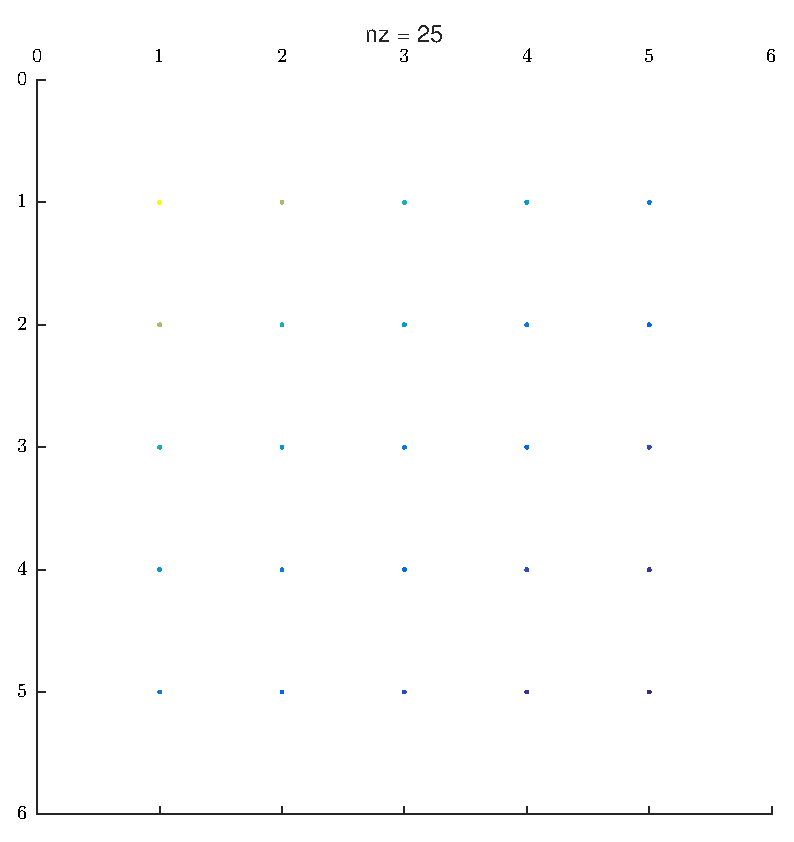
\includegraphics[width=4in]{math609_pa1_comp_example_3_n_5.eps}
	\caption{Matrix  at n = 5}
\end{center}
\end{figure}

\begin{figure}[!hbt]
\begin{center}
	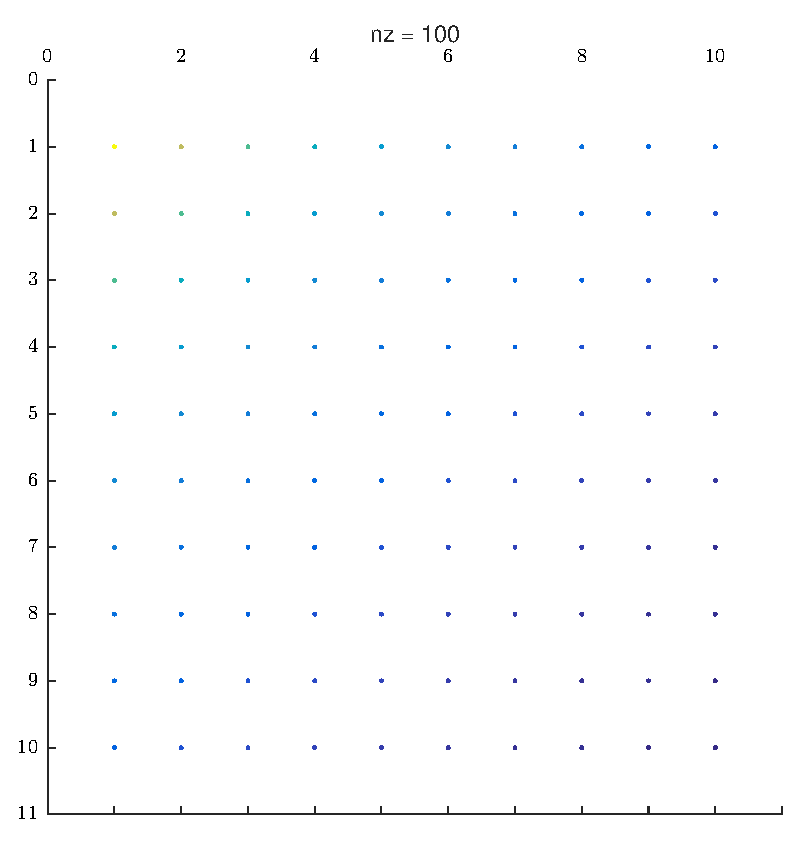
\includegraphics[width=4in]{math609_pa1_comp_example_3_n_10.eps}
	\caption{Matrix  at n = 10}
\end{center}
\end{figure}

\begin{figure}[!hbt]
\begin{center}
	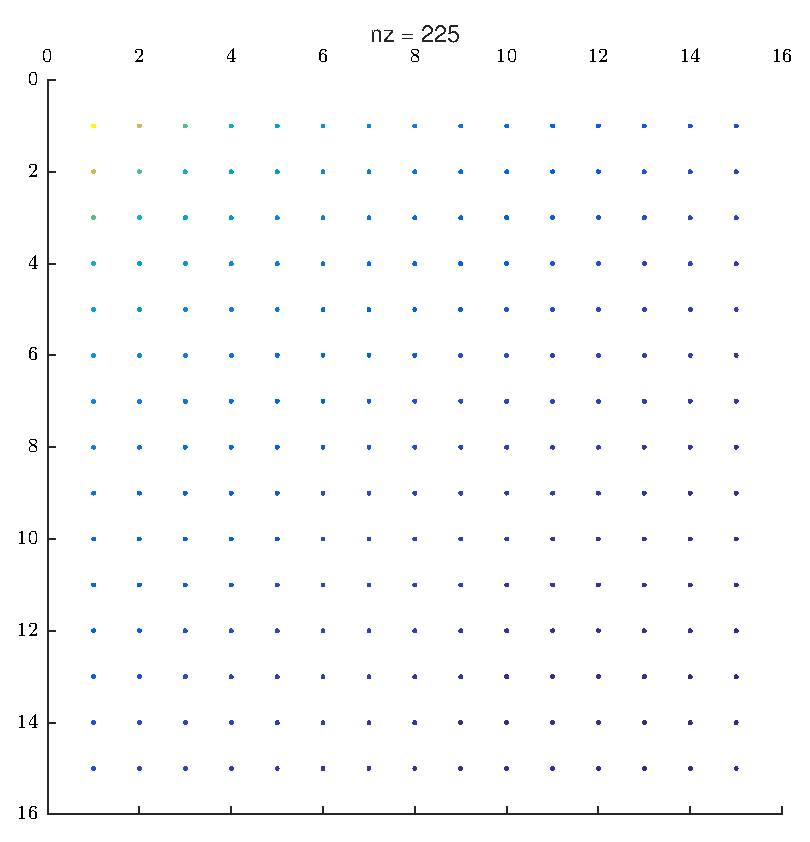
\includegraphics[width=4in]{math609_pa1_comp_example_3_n_15.eps}
	\caption{Matrix  at n = 15}
\end{center}
\end{figure}

\begin{figure}[!hbt]
\begin{center}
	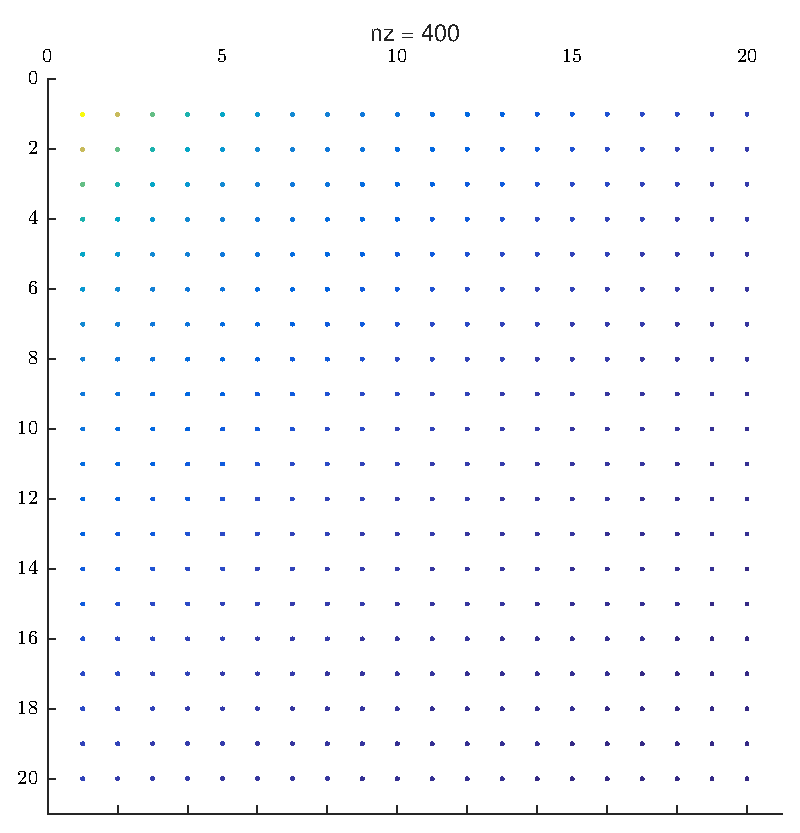
\includegraphics[width=4in]{math609_pa1_comp_example_3_n_20.eps}
	\caption{Matrix  at n = 20}
\end{center}
\end{figure}

\begin{figure}[!hbt]
\begin{center}
	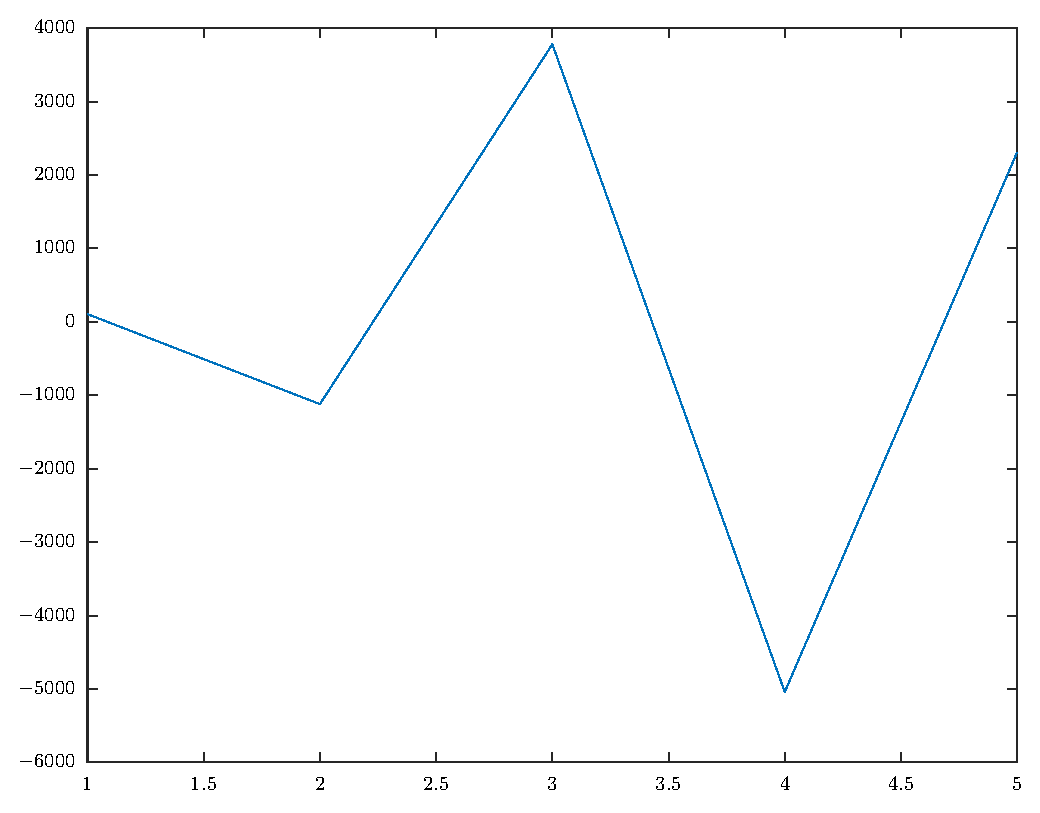
\includegraphics[width=4in]{math609_pa1_comp_example_3_n_5_.eps}
	\caption{Solution  at n = 5}
\end{center}
\end{figure}

\begin{figure}[!hbt]
\begin{center}
	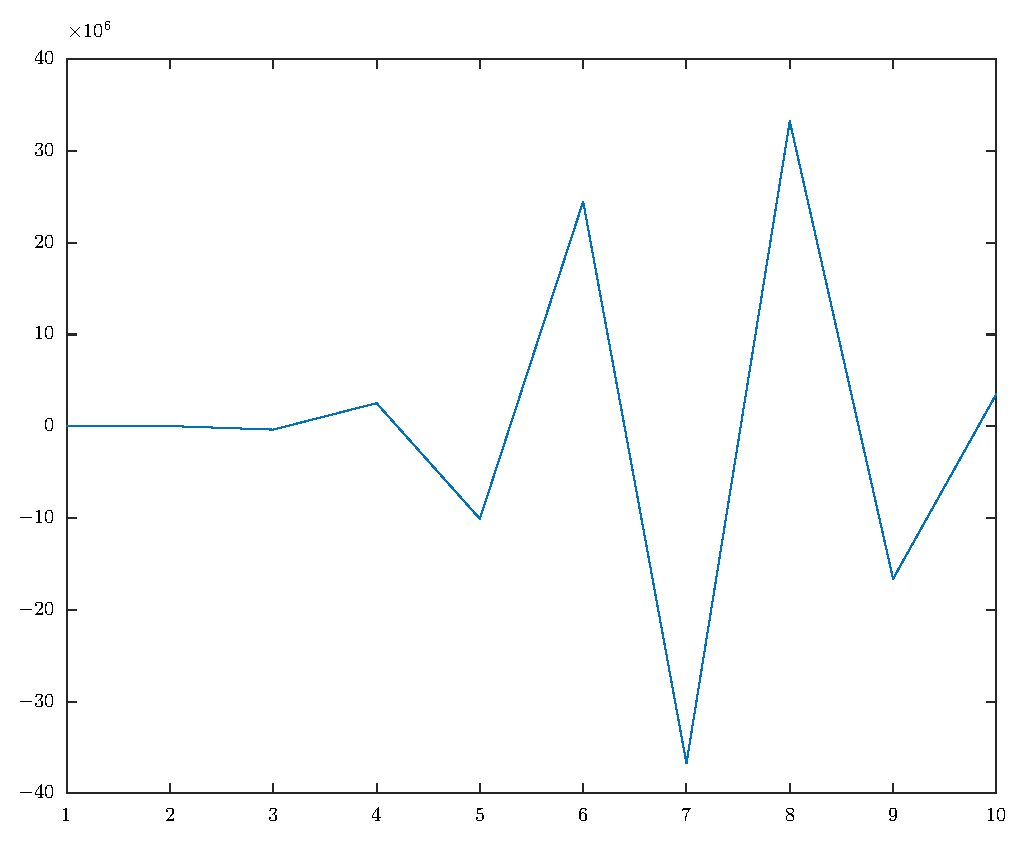
\includegraphics[width=4in]{math609_pa1_comp_example_3_n_10_.eps}
	\caption{Solution  at n = 10}
\end{center}
\end{figure}

\begin{figure}[!hbt]
\begin{center}
	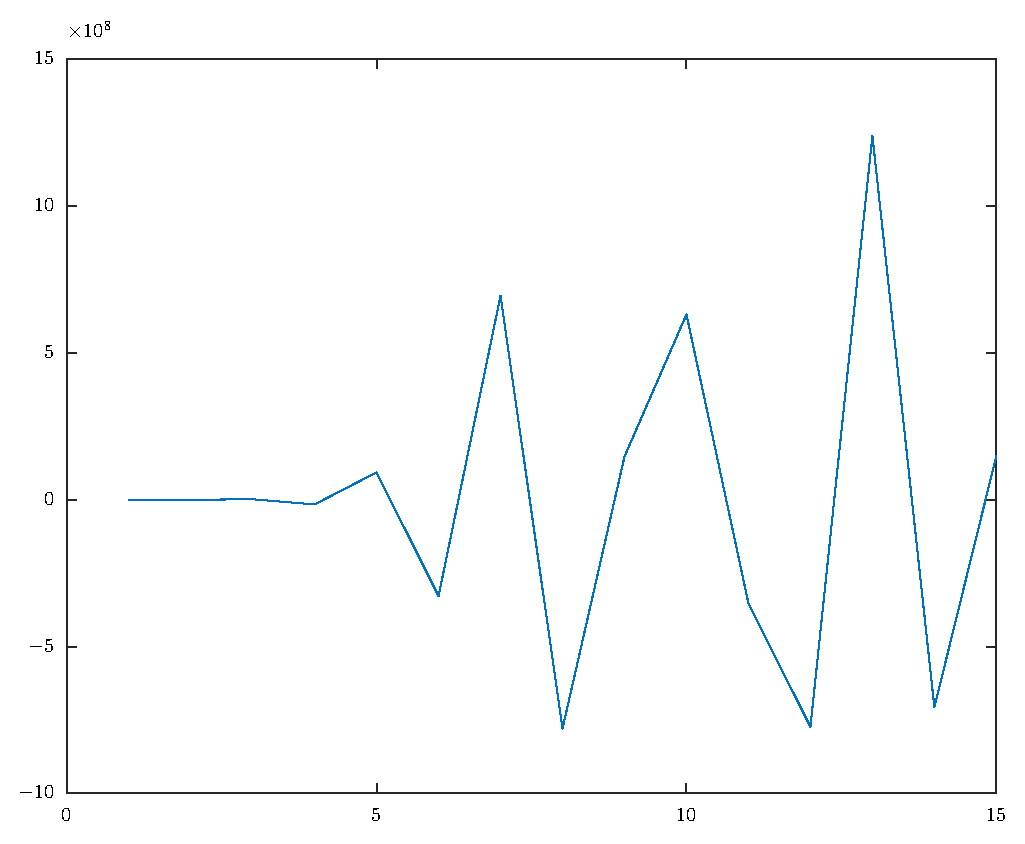
\includegraphics[width=4in]{math609_pa1_comp_example_3_n_15_.eps}
	\caption{Solution  at n = 15}
\end{center}
\end{figure}

\begin{figure}[!hbt]
\begin{center}
	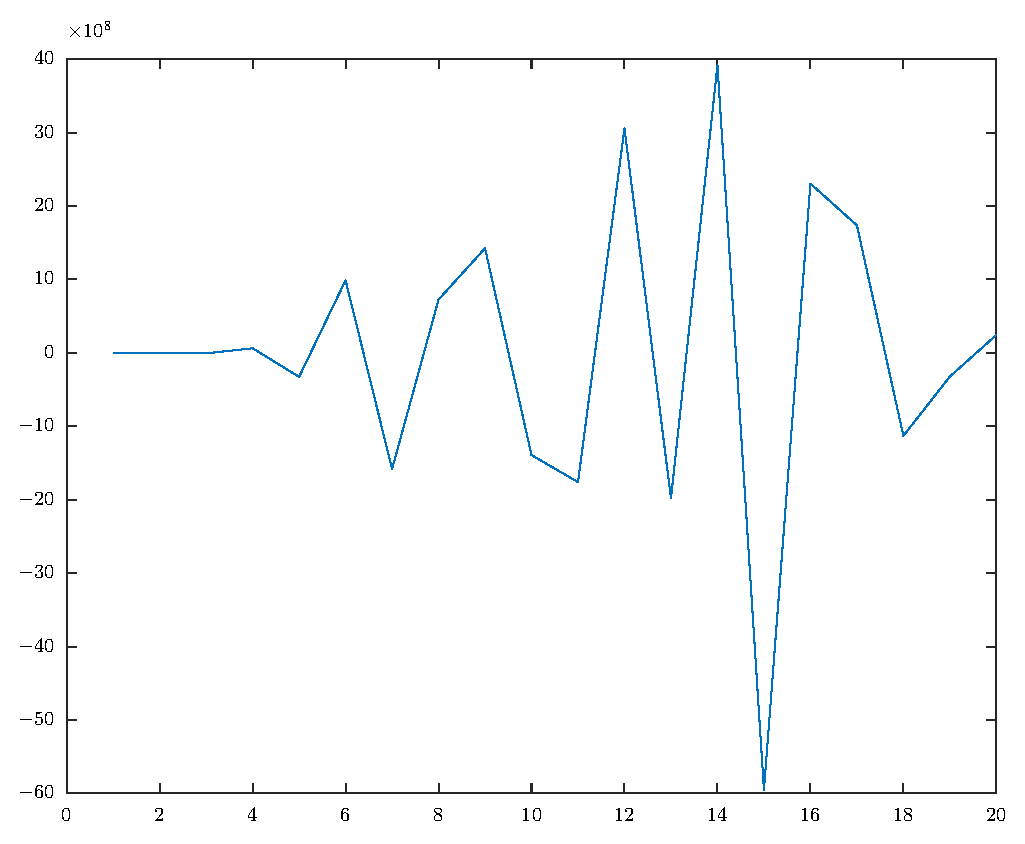
\includegraphics[width=4in]{math609_pa1_comp_example_3_n_20_.eps}
	\caption{Solution  at n = 20}

As can be seen, the solution becomes larger and diverges. Hence the system outputs a poor result.
\end{center}
\end{figure}


\end{document}








